\documentclass[a4paper,11pt]{article}
\usepackage[utf8]{inputenc}
\usepackage{graphicx}
\graphicspath{{immagini/}}
\usepackage{textcomp}
\usepackage{afterpage} 
\usepackage{afterpage} 
\usepackage{geometry}
\usepackage{booktabs}
\usepackage{amsmath}
\usepackage{amsfonts}
\usepackage{amssymb}
\usepackage{subfig}
\usepackage{geometry}
\usepackage{booktabs}
\usepackage{graphicx}
\usepackage{caption}
\usepackage{subfig}
\geometry{a4paper,top=3cm,bottom=3 cm,left=3.5cm,right=3.5cm,%
heightrounded,bindingoffset=5mm}
\usepackage{hyperref}
\newcommand{\HRule}{\rule{\linewidth}{0.5mm}}

\begin{document}
\begin{titlepage}
\begin{center}

% Upper part of the page. The '~' is needed because \\
% only works if a paragraph has started.
%\includegraphics[width=0.30\textwidth]{./immagini/logo.png}~\\[1cm]

\textsc{\LARGE Università degli studi di Padova}\\[1.5cm]

\textsc{\Large Physics Laboratory}\\[0.5cm]

% Title
\HRule \\[0.4cm]
{ \huge \bfseries Timing\\ [0.4cm] }

\HRule \\[1.5cm]

% Author and supervisor
\noindent
\begin{minipage}{0.4\textwidth}
\begin{flushleft} \large
\emph{Autori:}\\
Luca \textsc{Morselli}\\
Andrea \textsc{Raggio}\\
\end{flushleft}
\end{minipage}%
\begin{minipage}{0.4\textwidth}
\begin{flushright} \large
\emph{Docenti:} \\
Luca \textsc{stevanato}\\
Francesco \textsc{recchia}\\
\end{flushright}
\end{minipage}

\vfill

% Bottom of the page
{\large \today}

\end{center}
\end{titlepage}

\section*{Goals of the experiment}
In this experiment we want to achieve the following goals:

\begin{itemize}
\item Energy calibration of the organic scintillators and
calculation of the energy resolution from the analysis of
the Compton edge.
\item Optimization of the external delay of the analogue
CFTD to obtain the best time resolution.
\item Study the time resolution behaviour as a function of the
energy.
\item Comparison between the timing resolutions obtained
from analogue and digital treatment of the signals.
\item Measurement of the speed of light. 
\end{itemize}

\section*{Energy Calibration}

In this experiment we have used  two cylindrical organic scintillators EJ-228, with a 5 cm diameter and 5 cm thickness. 
Due to the organic composition of our detectors the photo-electric cross-section of its constituents is negligible for the energy used in laboratory. Furthermore due two the limited size of the detectors total absorbtion through multiple compton scattering is negligible too. The detectors response will be dominated by the individual Compton interaction, the result in the energy spectrum is a continuous distribution that corresponds to different angles of interaction. This can be seen in the spectra acquired with the $•^{22}$Na source (Fig. \ref{fig: uncalibrated energy spectra}).

\smallskip
\begin{figure}[h!]
\centering
\subfloat[][\emph{Detector \#1 spectrum}.]
   {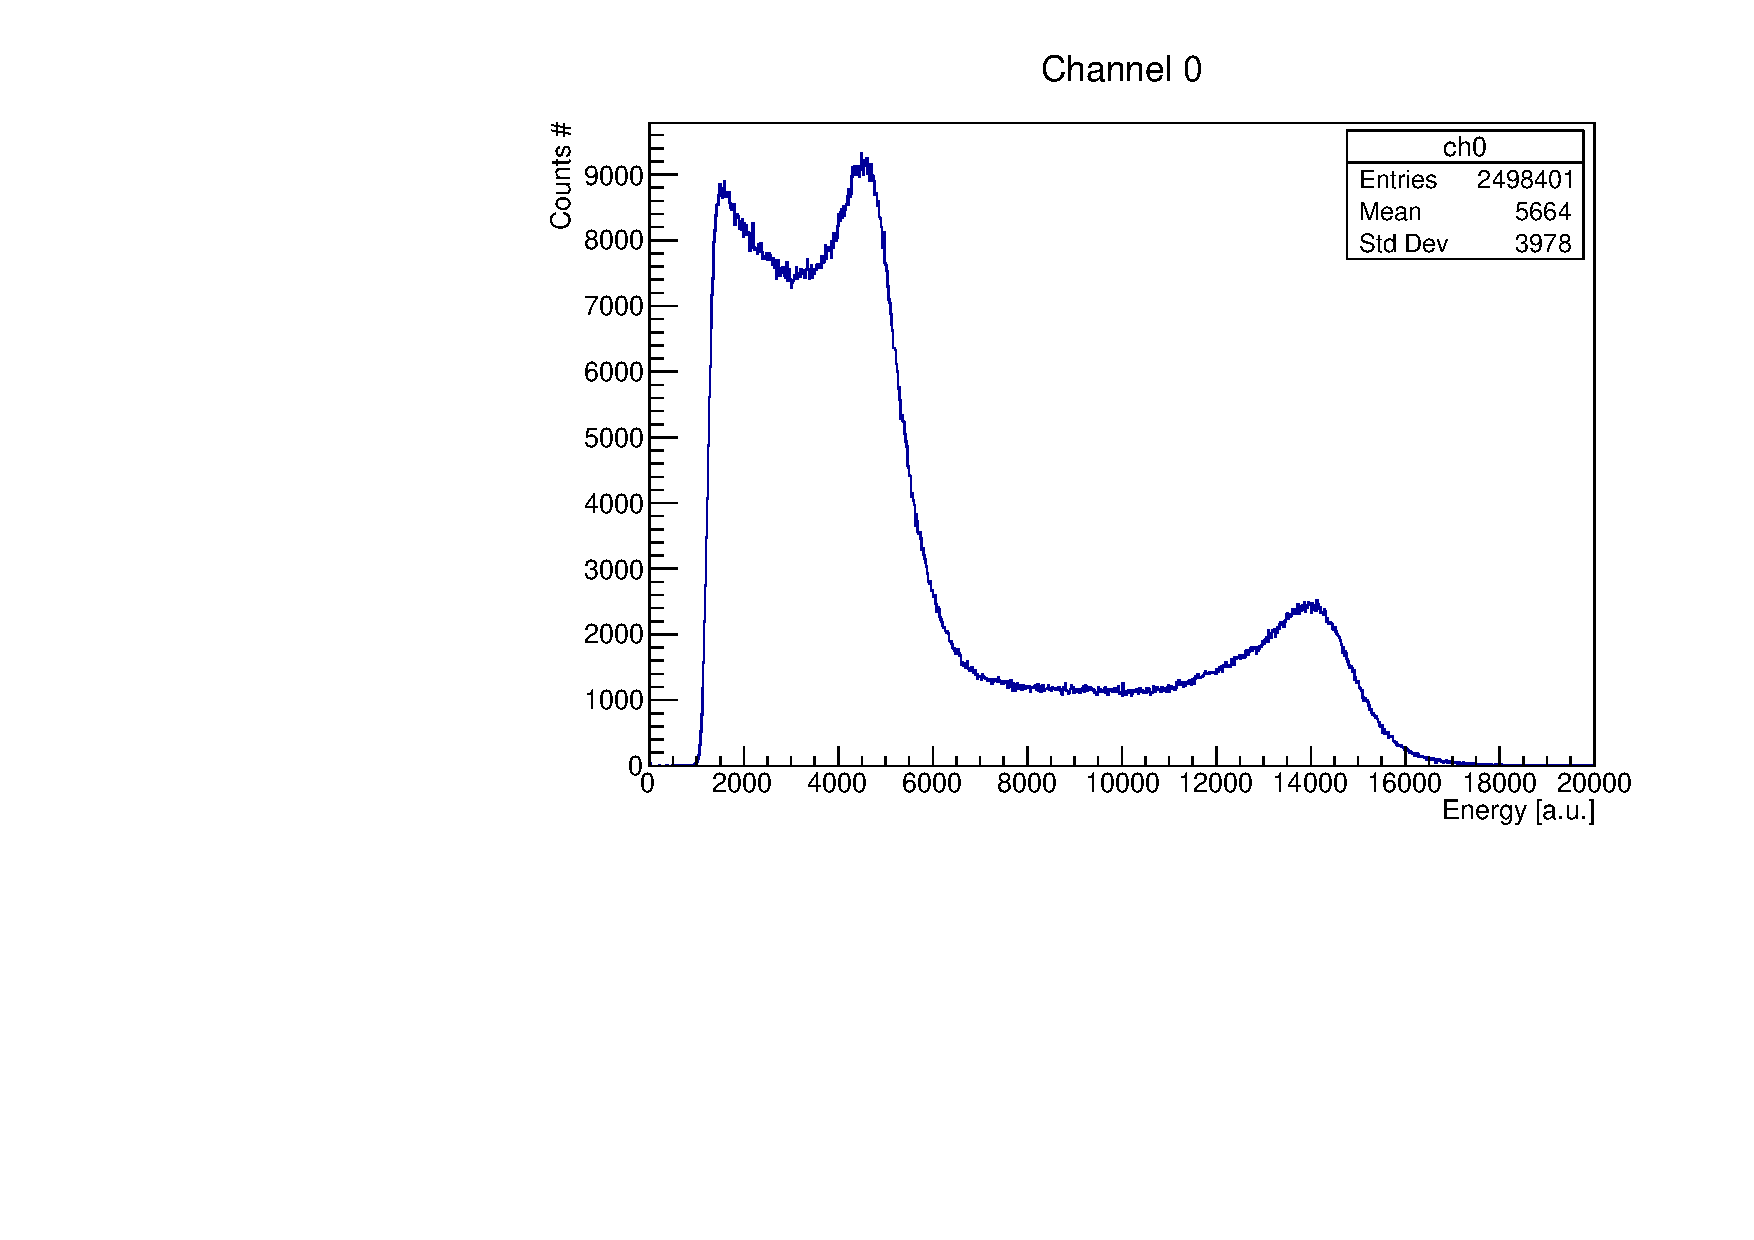
\includegraphics[width=.45\textwidth]{d1_spectrum_qlong}} \quad
\subfloat[][\emph{Detector \#2 spectrum}.]
   {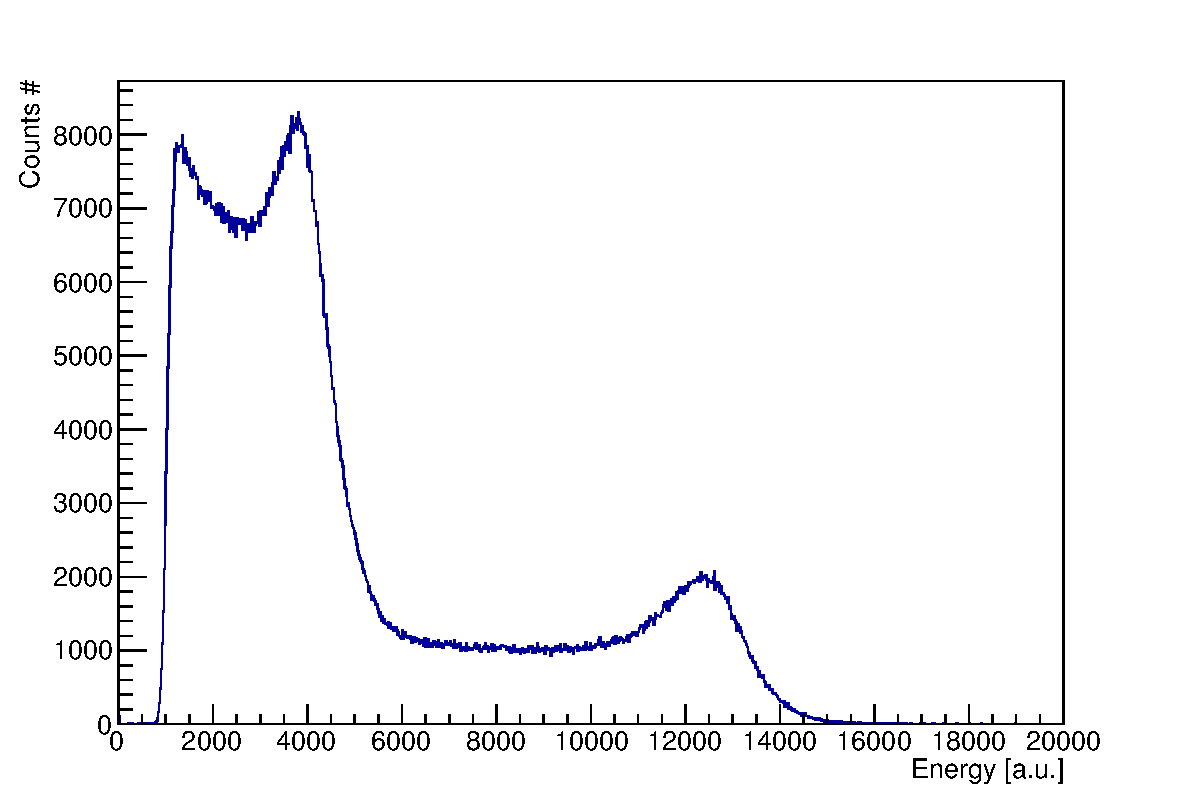
\includegraphics[width=.45\textwidth]{d2_spectrum_qlong}} \\
\caption{Detectors spectra (not calibrated).}
\label{fig: uncalibrated energy spectra}
\end{figure}
\clearpage
\noindent The finite resolution of our detectors result in a shift towards lower energies depending on the detector resolution (Fig. \ref{fig: smeared spectra}).
\begin{figure}[h!]
\centering
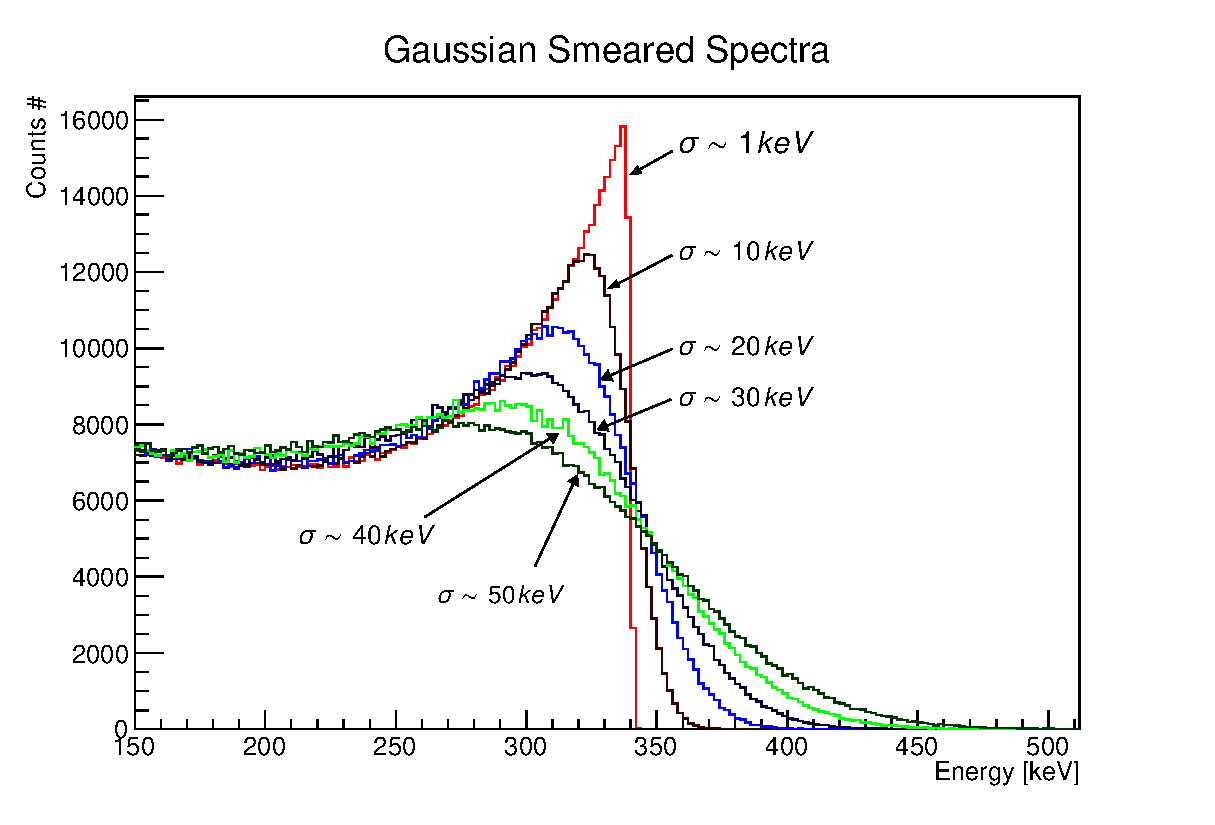
\includegraphics[width=0.8\textwidth]{smeared_spectra}
\caption{Gaussian smeared spectra at different $\sigma$ for 511 keV photon.}
\label{fig: smeared spectra}
\end{figure}


\noindent In order to obtain the energy calibration parameters we have to generate several smeared spectra using the Klein-Nishina cross-section for Compton Scattering:
\begin{equation*}
\dfrac{d\sigma}{dT} = \dfrac{\pi r_e^2}{m_ec^2\alpha^2}\left(2+\dfrac{s^2}{\alpha^2(1-s)^2}+\dfrac{s}{1-s} \left(s-\dfrac{2}{\alpha}\right) \right)
\end{equation*}
for $511$ keV and $1275$ keV respectively. Then we have to subtract the Compton background from acquired spectra in order to search for Compton edge position (Fig. \ref{fig: compton back}).
\begin{figure}[h!]
\centering
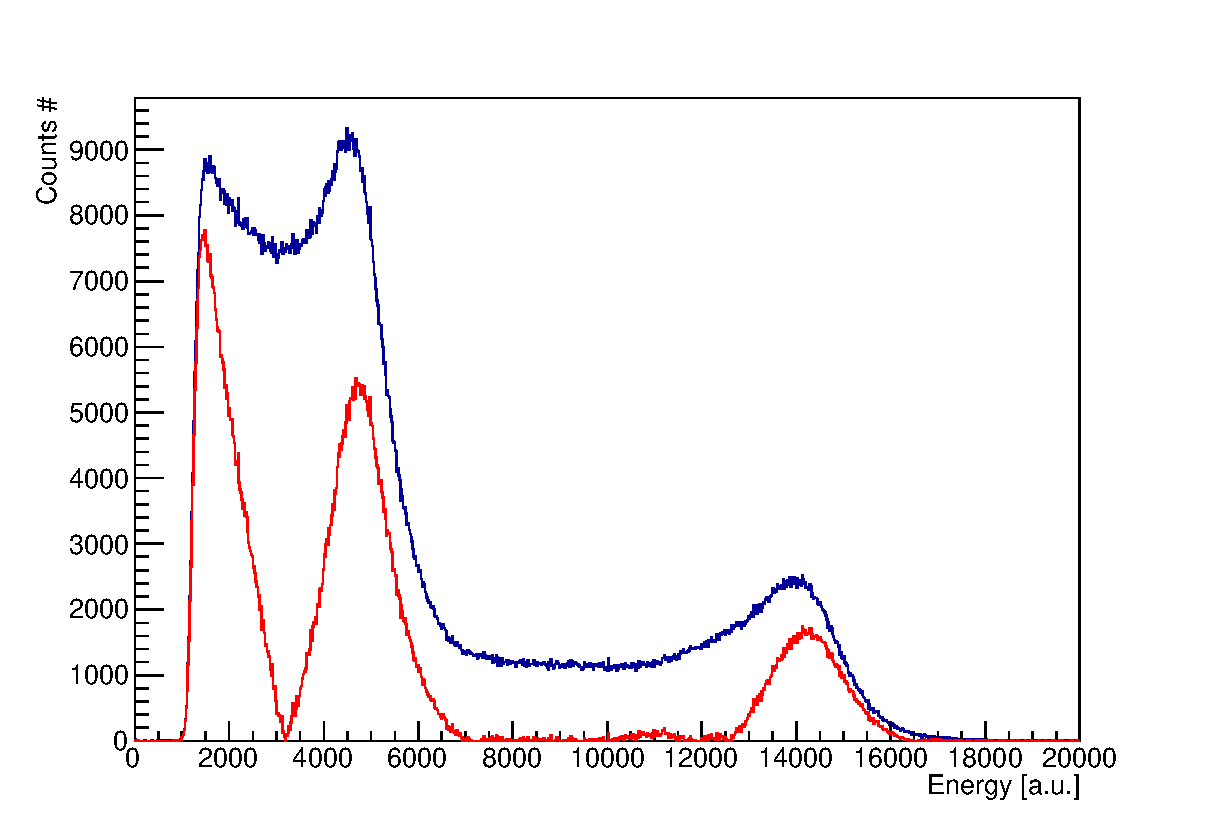
\includegraphics[width=0.8\textwidth]{spectra_vs_background.eps}
\caption{Acquired Spectra (blue). Spectra with subtracted Compton background (red).}
\label{fig: compton back}
\end{figure}

\noindent Once we have the compton edge position we have to loop on every previous generated smearing and calculating the $\chi^2$ between experimental spectrum and gaussian smeared one selecting the smearing with the $\sigma$ that led to minimum $\chi^2$. Once we have selected a proper $\sigma$ we have also the corresponding shift of the Compton Edge that we have to use in order to calibrate our detector.

\begin{figure}[h!]
\centering
\subfloat[][\emph{Detector \#1 spectrum}.]
   {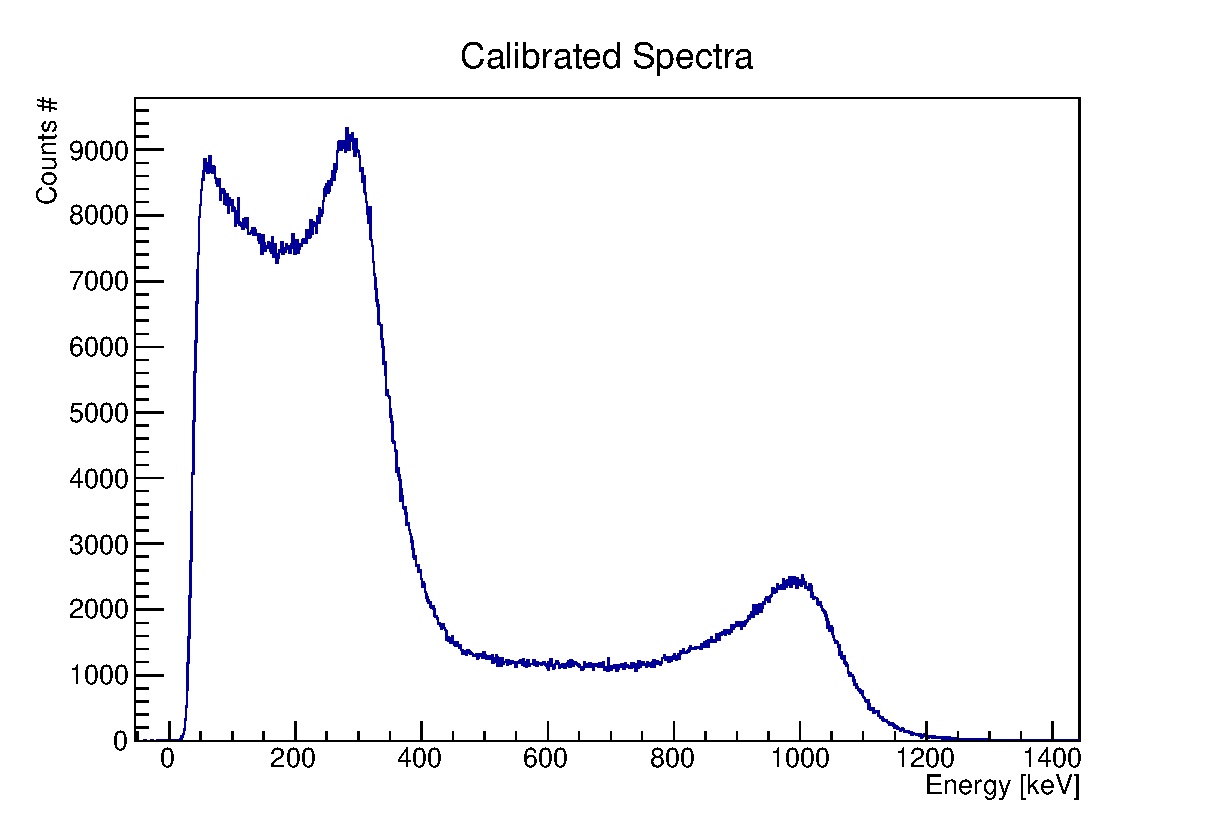
\includegraphics[width=.45\textwidth]{calibrated_spectra_d1}} \quad
\subfloat[][\emph{Detector \#2 spectrum}.]
   {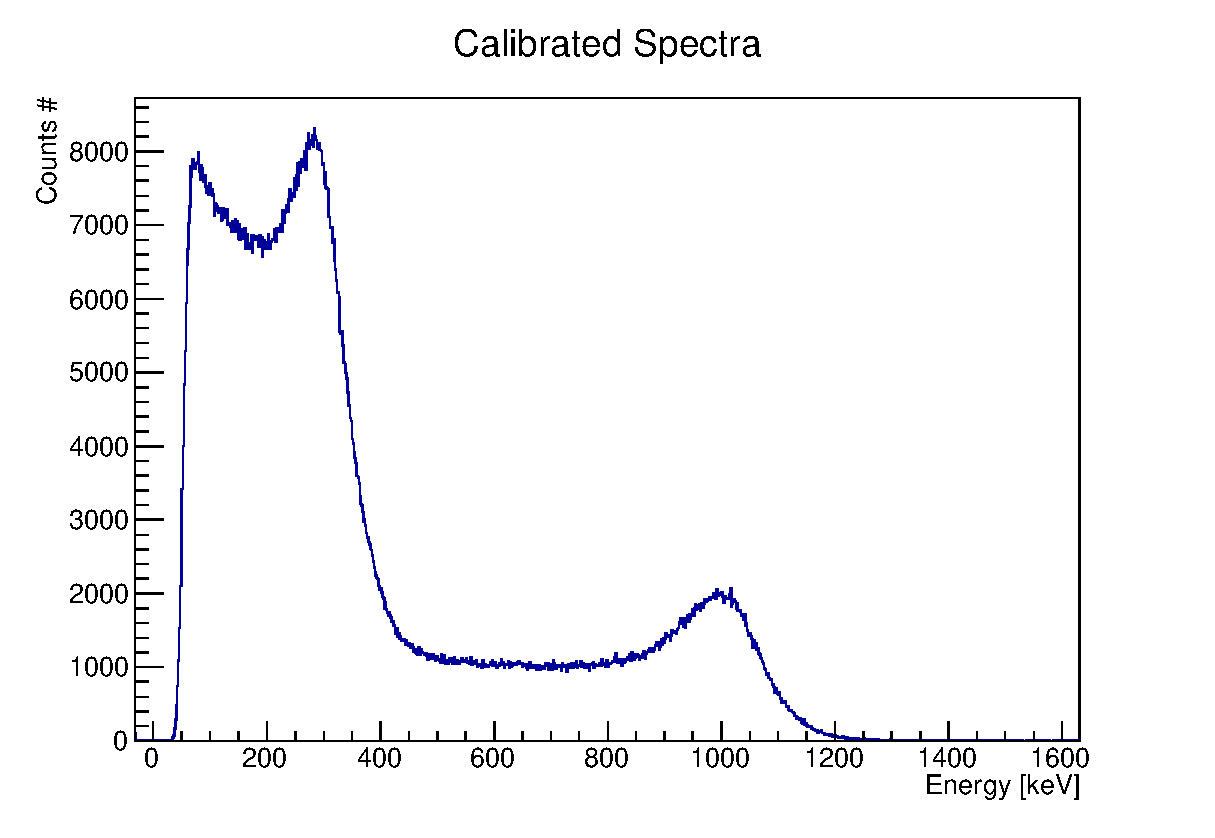
\includegraphics[width=.45\textwidth]{calibrated_spectra_d2}} \\
\caption{Calibrated detectors spectra.}
\label{fig: calibrated energy spectra}
\end{figure}

\begin{table}[h!]
\centering
\begin{tabular}{ccc}
\toprule
\toprule
Photon Energy [keV] & $\sigma$ [keV] & C.E. shifting [keV] \\
\midrule
511 & 34& 40.66 \\
1275 & 40 & 52.15\\
\bottomrule
\bottomrule
\end{tabular}
\caption{$\sigma$ and C.E. shift for detector \#1.}
\end{table}

\begin{table}[h!]
\centering
\begin{tabular}{ccc}
\toprule
\toprule
Photon Energy [keV] & $\sigma$ [keV] & C.E. shifting [keV] \\
\midrule
511 & 28 & 34.66 \\
1275 & 40 & 52.15\\
\bottomrule
\bottomrule
\end{tabular}
\caption{$\sigma$ and C.E. shift for detector \#2.}
\end{table}
\begin{table}[h!]
\centering
\begin{tabular}{ccc}
\toprule
\toprule
Detector & a [keV/channel] & b [keV] \\
\midrule
\#1 &  0.0748945$\pm$ & -54.2511$\pm$ \\
\#2 & 0.083215$\pm$ & -32.6856$\pm$ \\
\bottomrule
\bottomrule
\end{tabular}
\caption{Calibration parameters.}
\end{table}



%\begin{figure}[h!]
%\centering
%\subfloat[][\emph{Low energy Compton Edge}.]
%   {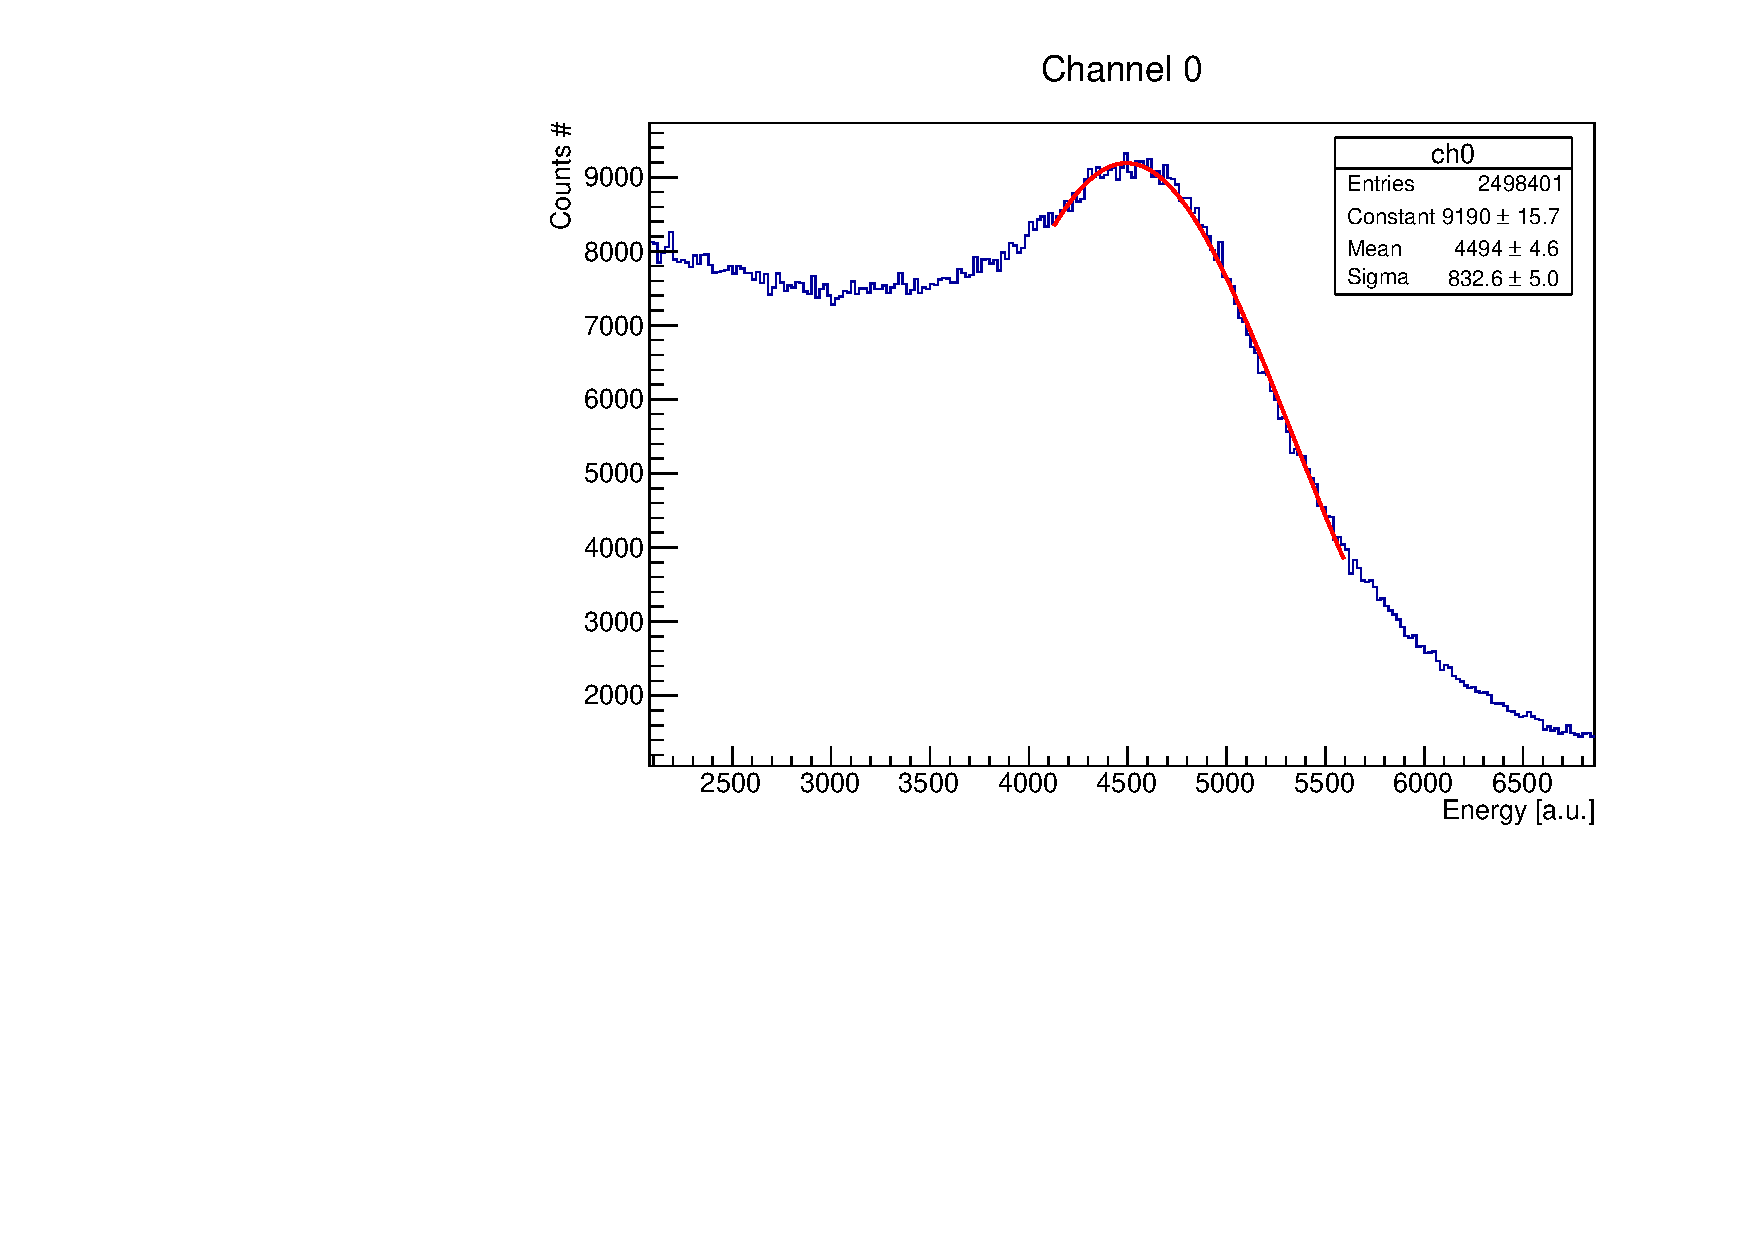
\includegraphics[width=.45\textwidth]{fit_511_d1}} \quad
%\subfloat[][\emph{High energy Compton Edge}.]
%   {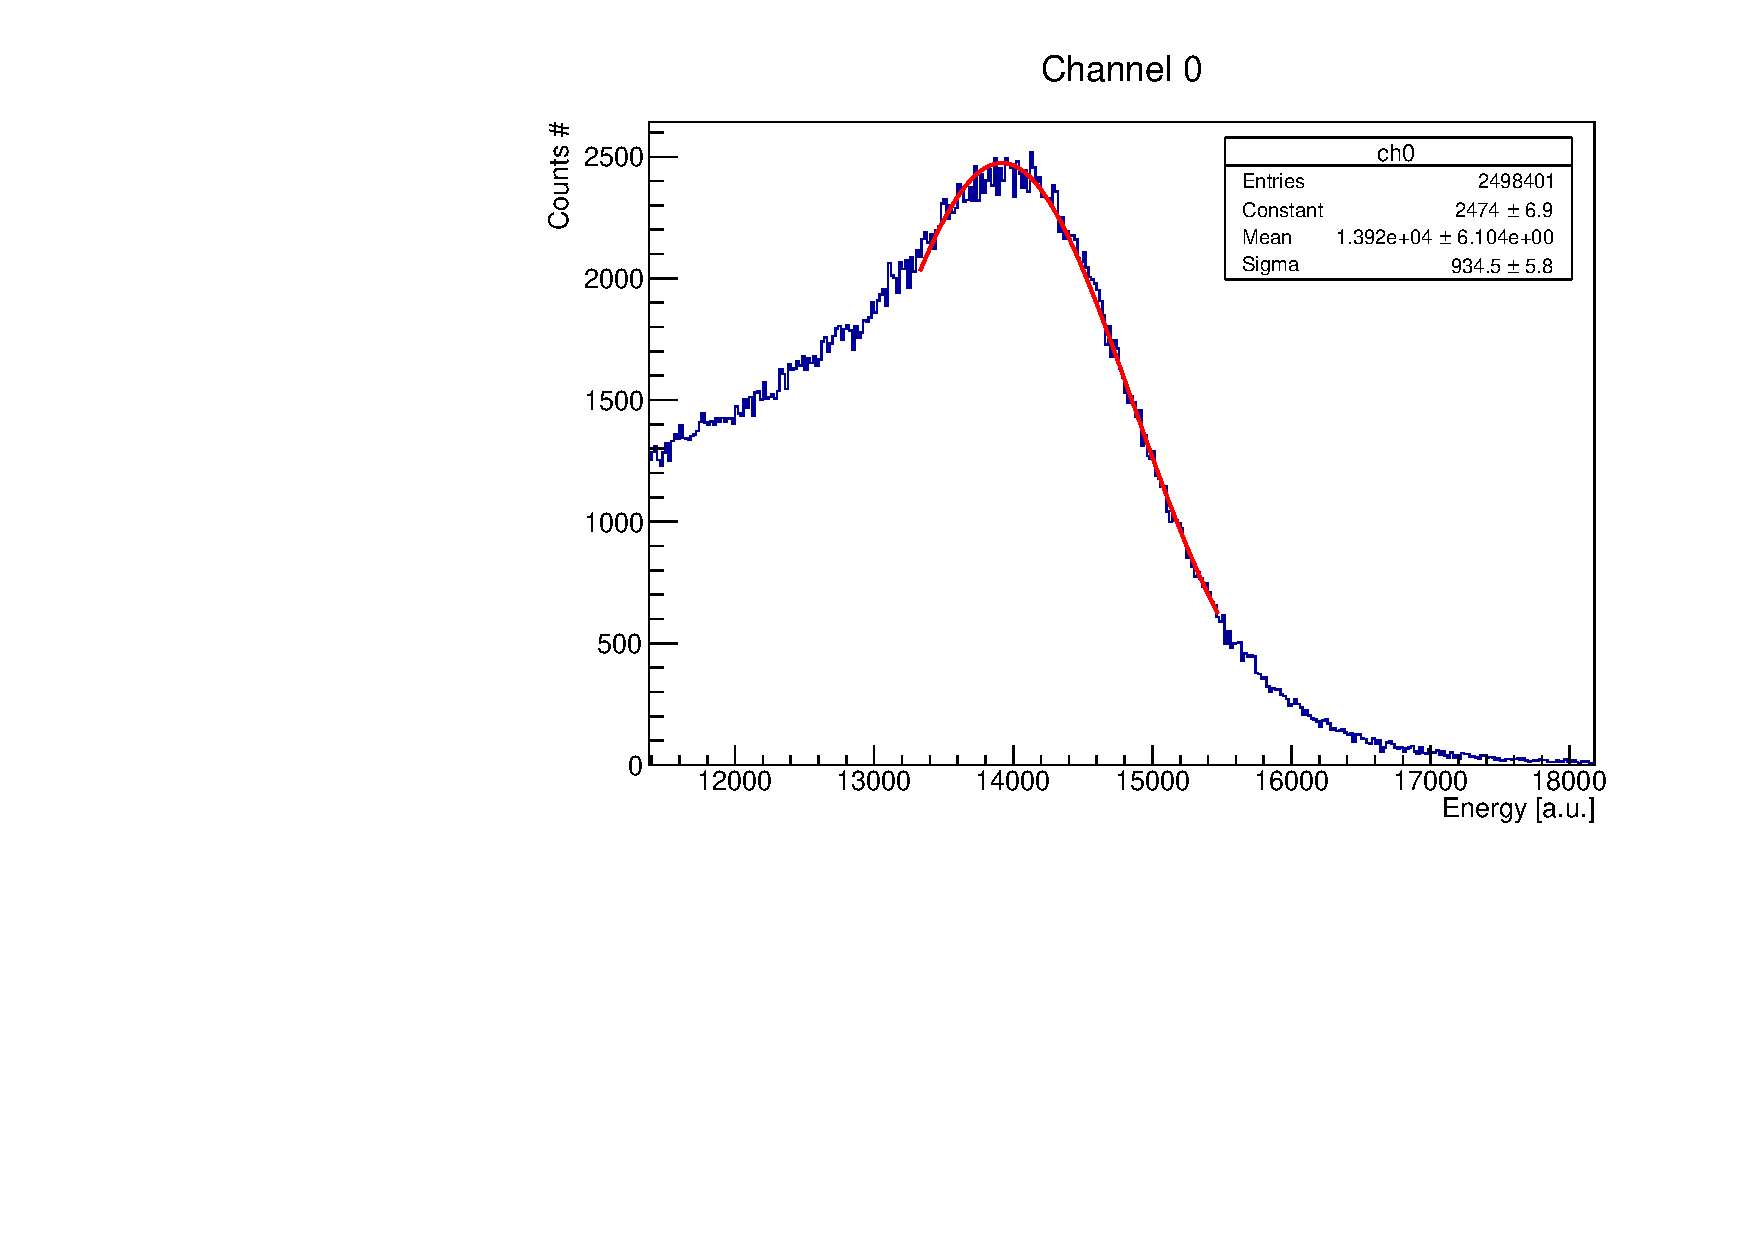
\includegraphics[width=.45\textwidth]{fit_1275_d1}} \\
%\caption{Compton Edge for Detector \#1 .}
%\end{figure}
%
%\begin{figure}[h!]
%\centering
%\subfloat[][\emph{Low energy Compton Edge}.]
%   {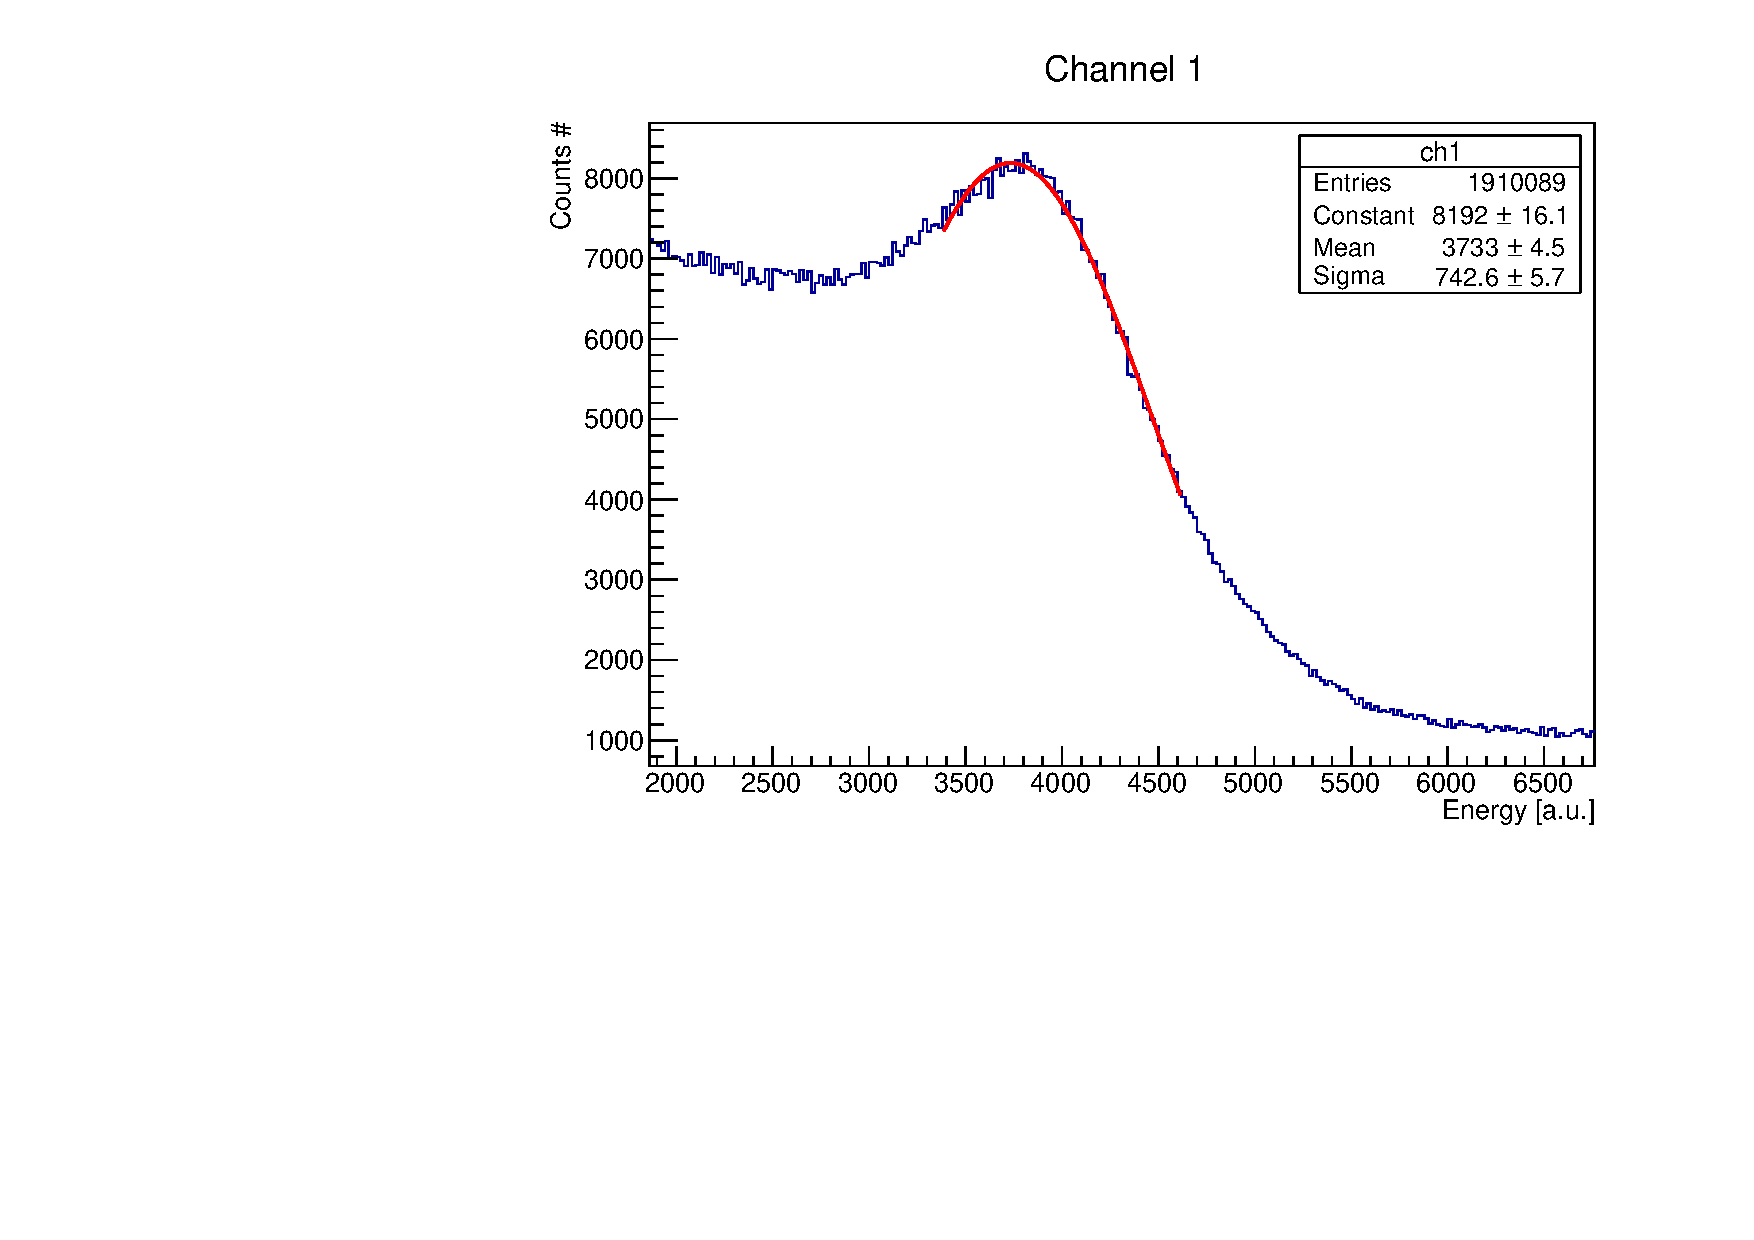
\includegraphics[width=.45\textwidth]{fit_511_d2}} \quad
%\subfloat[][\emph{High energy Compton Edge}.]
%   {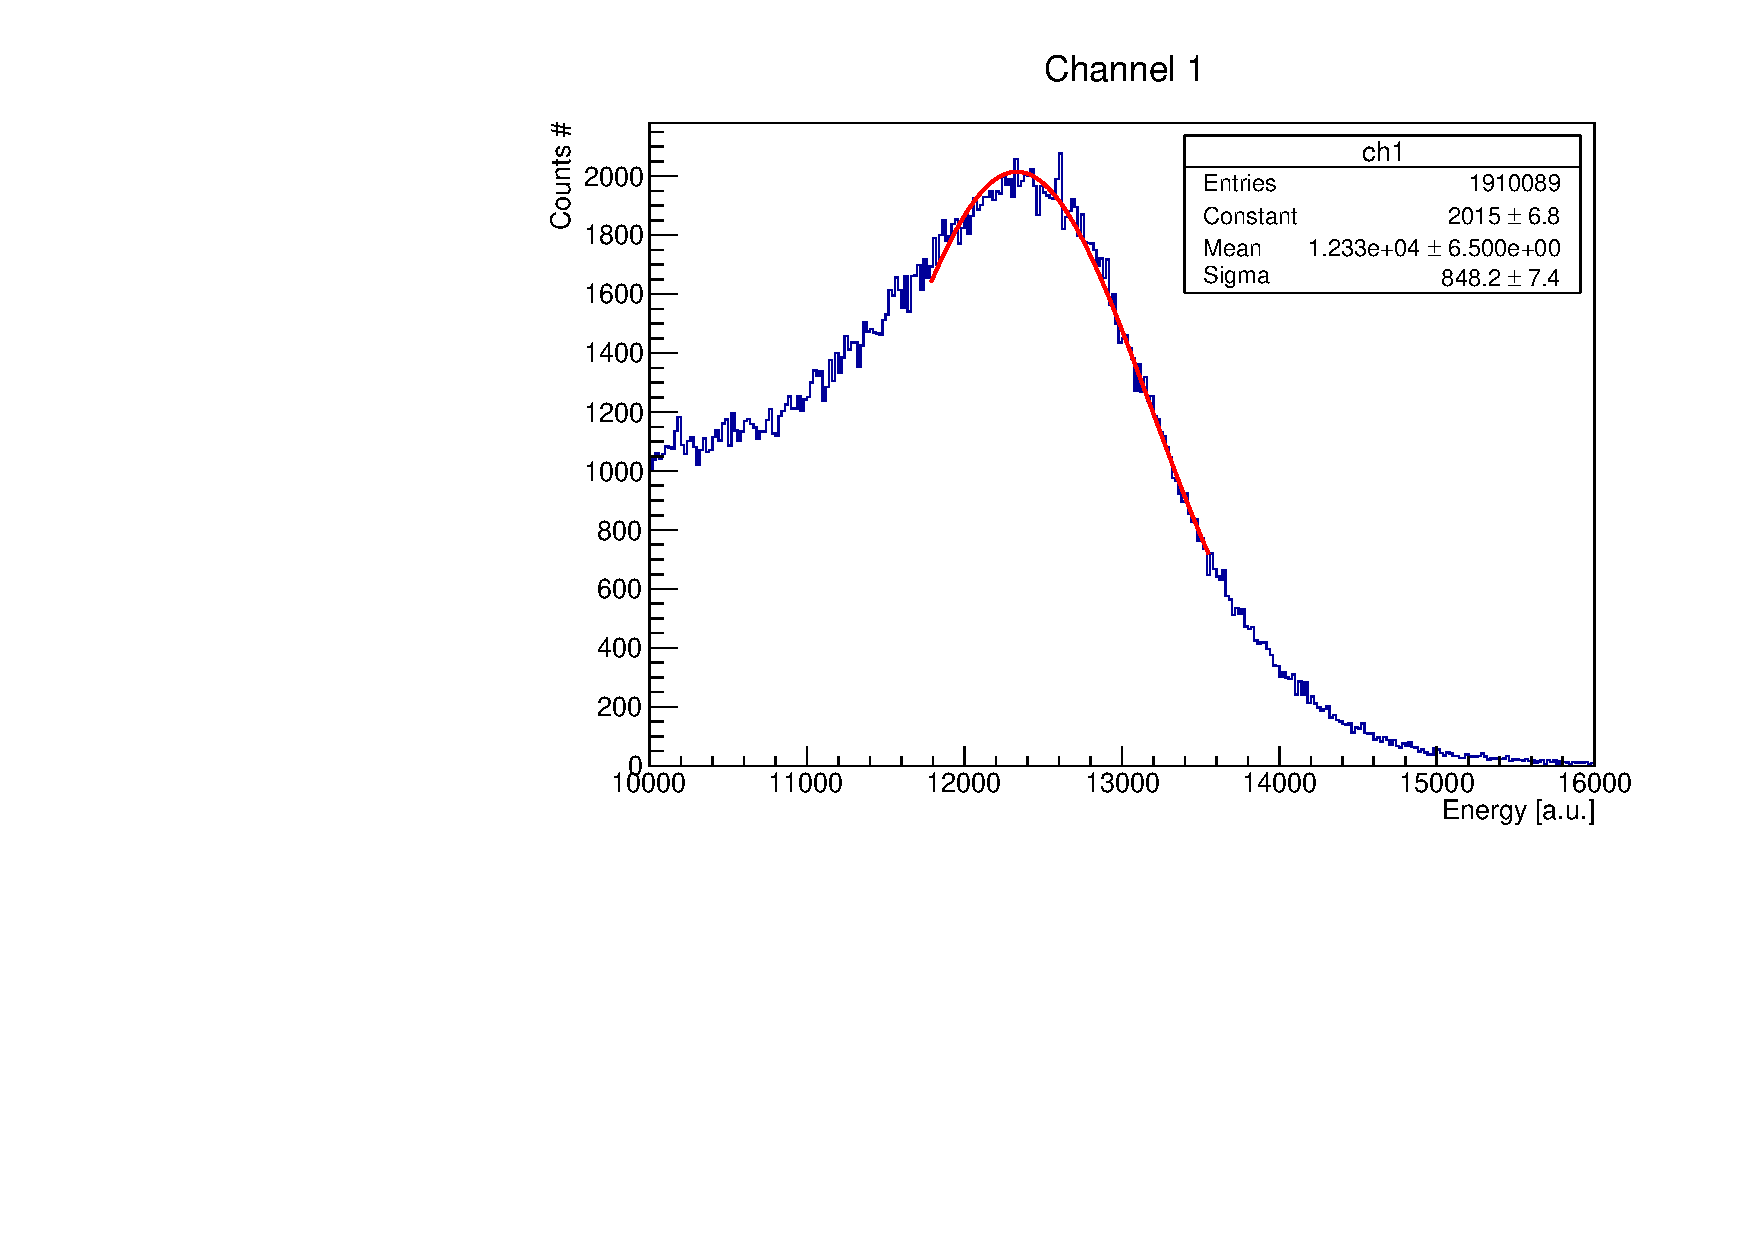
\includegraphics[width=.45\textwidth]{fit_1275_d2}} \\
%\caption{Compton Edge for Detector \#2 .}
%\end{figure}
%
\clearpage
\section*{TAC calibration}
In order to calibrate the TAC we have acquired data using auto coincidence between a detector signal and itself. By changing the delay in the delay unit we have obtained the spectra in the Fig. \ref{fig: uncalibrated TAC}. Then using TSpectrum we have found the peaks centroid and fit the using a linear function (Fig. \ref{fig: fit tac}). The calibrated spectra is shown in Fig. \ref{fig: calibrated TAC}.
\begin{figure}[h!]
\centering
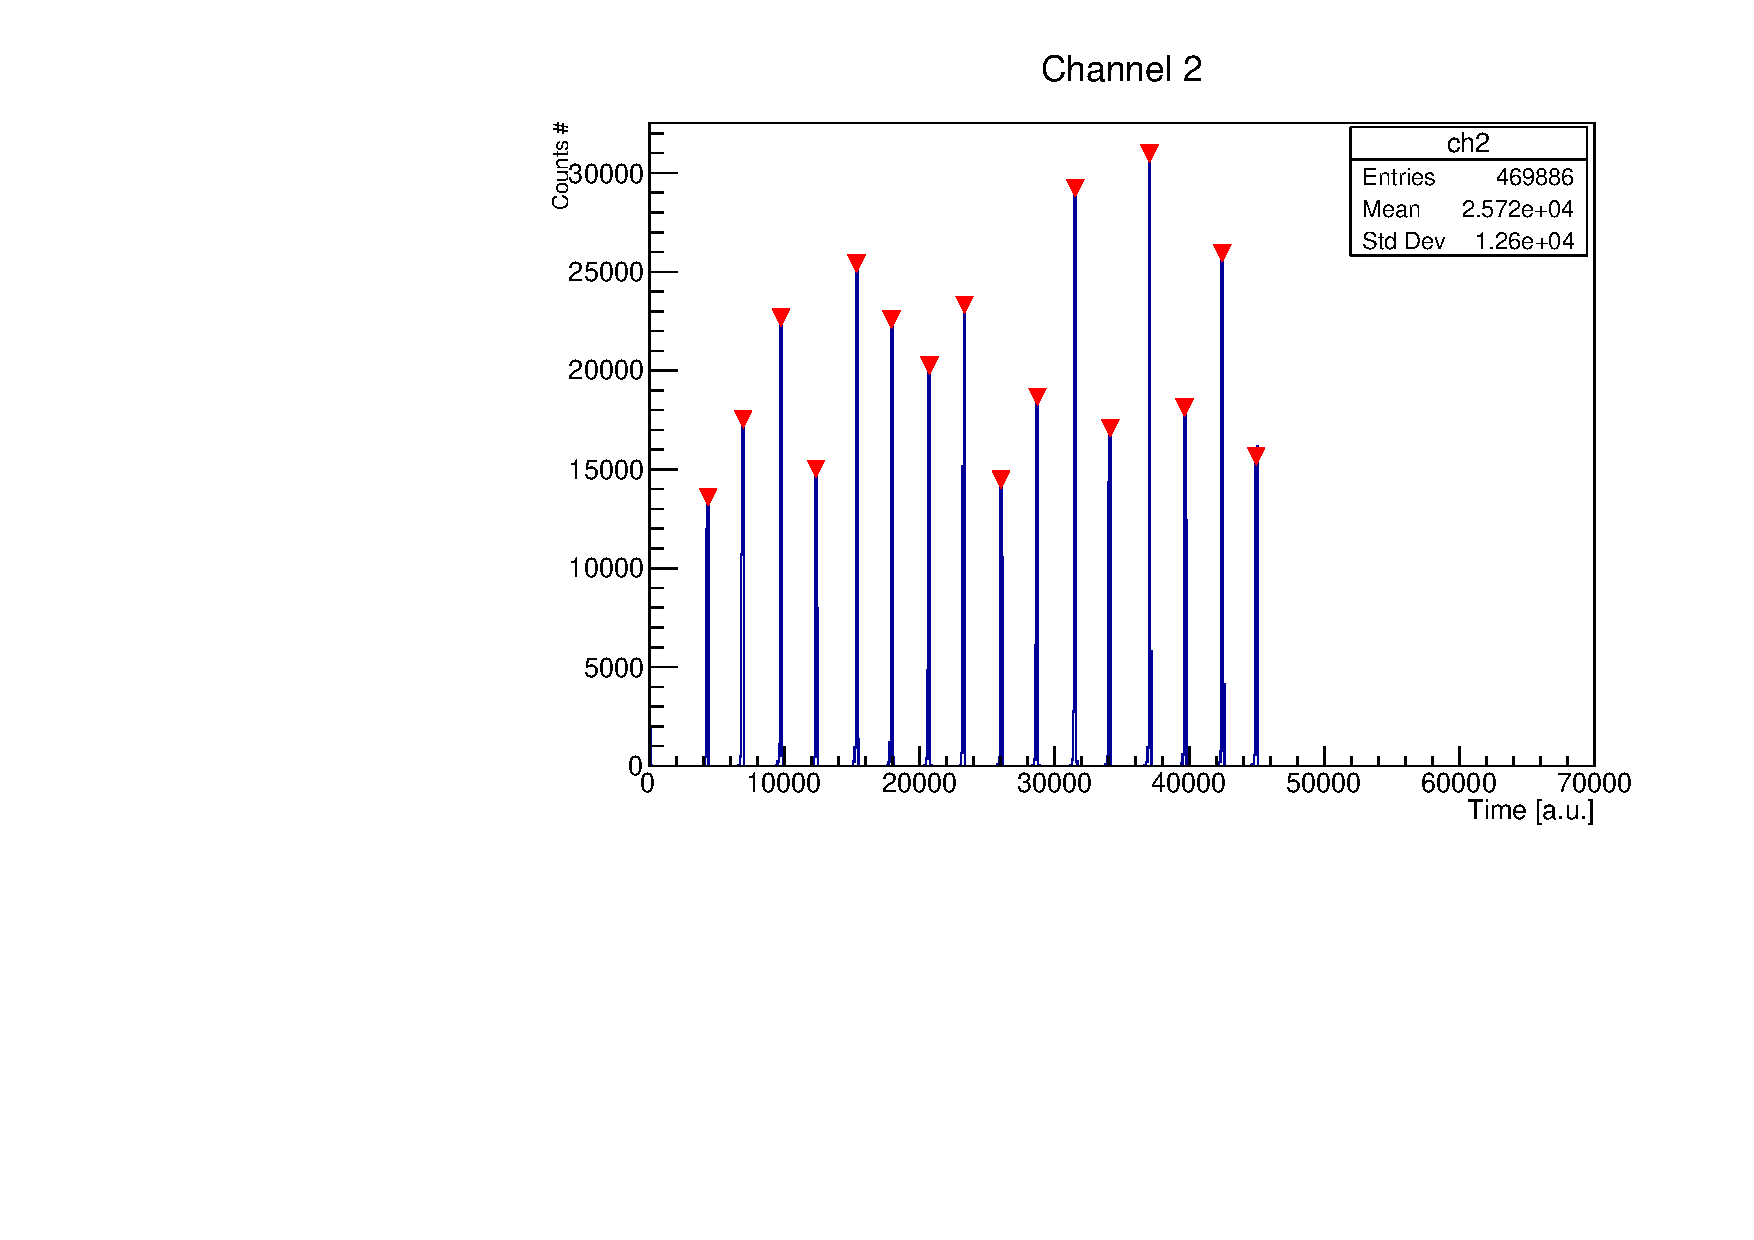
\includegraphics[width=0.8\textwidth]{tac_uncalibrated_spectrum.pdf}
\caption{TAC spectrum (not calibrated). Obtained with an autocoincidence.}
\label{fig: uncalibrated TAC}
\end{figure}


\begin{figure}[h!]
\begin{minipage}[b]{0.6\textwidth}
\centering
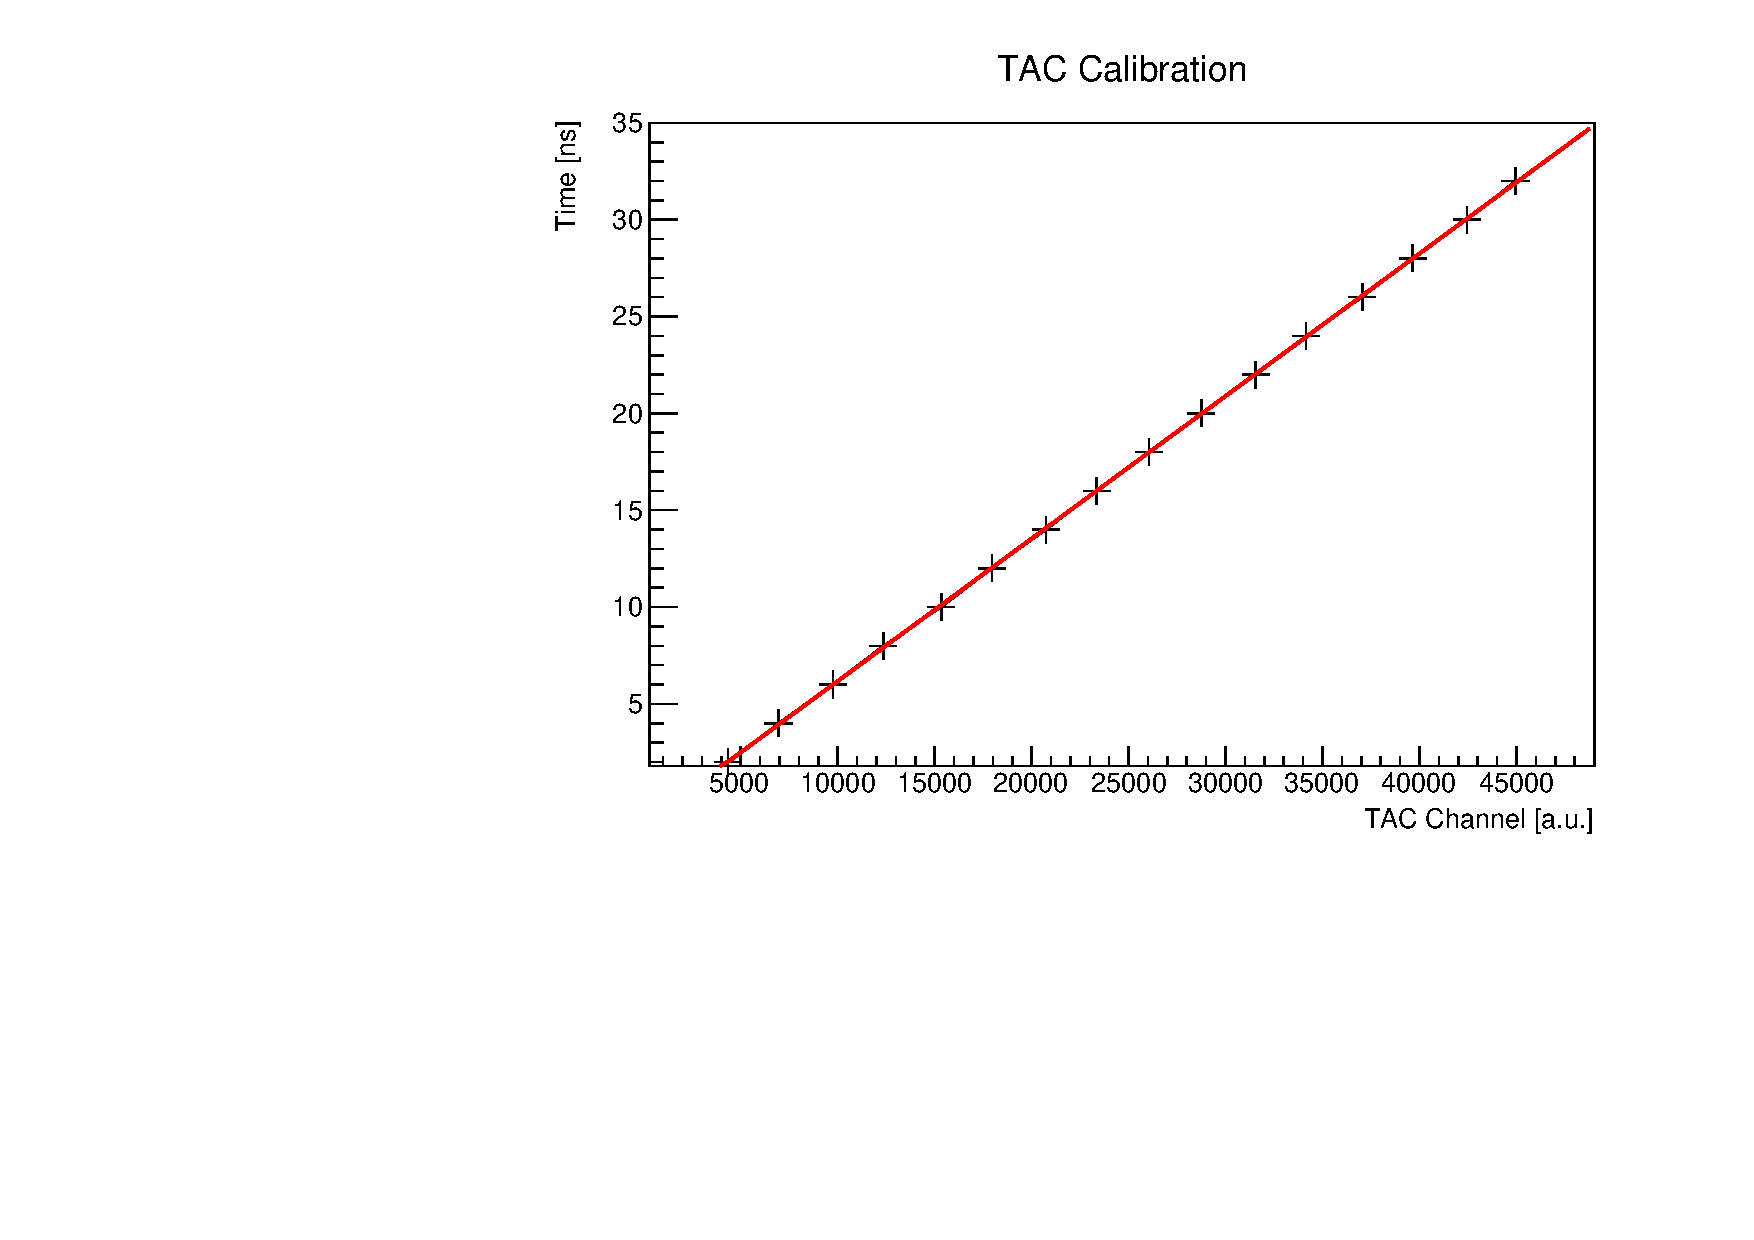
\includegraphics[width=\textwidth]{fit_calibrazione_tac}
\caption{Fit for TAC calibration.}
\label{fig: fit tac}
\end{minipage}
\hfill
\begin{minipage}[b]{0.45\textwidth}
\centering
\begin{tabular}{cc}
\toprule
\toprule
Parameter & Value \\
\midrule
p0     & -1.19 $\pm$  0.04 \\
p1     &  0.000736   $\pm$  0.000001\\
\bottomrule
\bottomrule
\end{tabular}
\vspace{1.5cm}
\caption{Fit parameters.}
\end{minipage}

\end{figure}

\begin{figure}[h!]
\centering
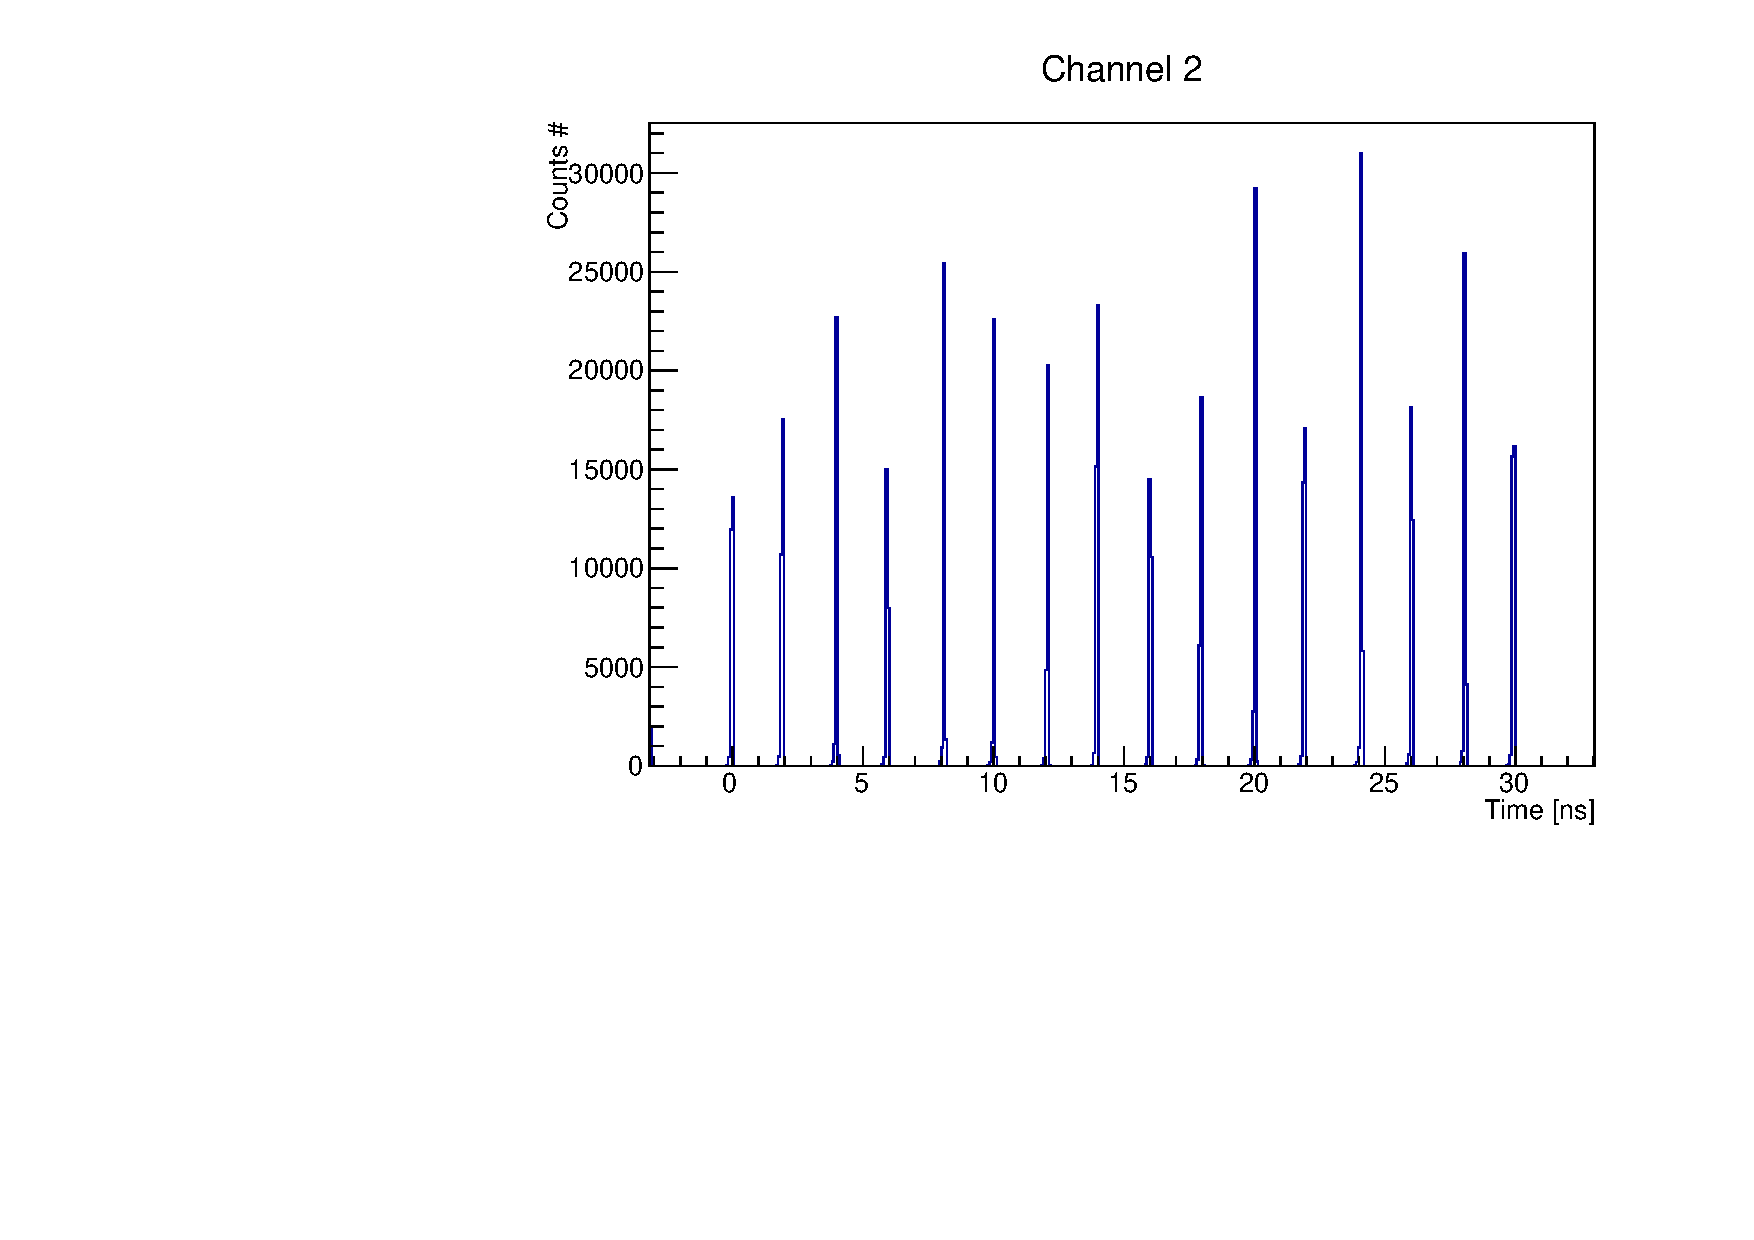
\includegraphics[width=0.8\textwidth]{tac_calibrato}
\caption{Calibrated TAC spectrum. }
\label{fig: calibrated TAC}
\end{figure}
\clearpage
\section*{External delay optimization}

\section*{Time resolution behaviour as a function of energy}
In order to study the time resolution dependence as a function of the energy we have used a different radioacive source, $^{60}$Co. This source is chosen because of its high energy Compton Edge (1 MeV) that allow us to study the energy dependence up to this energy. 

\noindent By imposing a lower energy threshold starting from 100 keV to 1000 keV we are able to plot the time resolution as a function of the lower energy threshold (Fig. ).

\noindent We can also proceed in a slightly different way. Instead of setting a lower energy threshold we can select energy windows with 100 keV of width and plotting the time resolution in function of the energ mid-energy (Fig. ).


% Dobbiamo commentare i risultati dopo le misure e 
% scrivere qual è la differenza tra soglie e finestre

\end{document}
